\chapter{Applications}
\label{chap:apps}

As mentioned in previous chapters, the SSaaS model can be utilized
across a range of existing and proposed applications. In each case,
the model allows users to reduce the trust they must place in any
single third party while retaining support for popular use cases
today. I present several potential SSaaS applications in this chapter.

\section{Storage}

One of the primary applications of the SSaaS model is to secure
storage systems, both local and hosted. These applications are all
variations on the previously discussed encrypted data + SSaaS-backed
keys model. In such applications, users handle the encrypting and
decryption of data locally, only sending encrypted data to third
parities or storing it on high risk devices. In order to ensure that
such client-side encryption does not break traditional features
associated with cloud and mobile data storage, clients store the
associated encryption keys with one or more Secret Storage Providers.

\subsection{Cloud File Sync/Storage}

\begin{figure}[t]
  \centering
  \includegraphics[height=200px]{./figs/out/App-FileStore.pdf}
  \caption{SSaaS-Backed Cloud File Storage System}
  \label{fig:apps-filestore}
\end{figure}

Building on the original motivating example in this proposal, using
Dropbox without trusting Dropbox with plain-text user data, we can
construct an SSaaS-backed cloud sync and storage
client. Figure~\ref{fig:apps-filestore} illustrates this
application. As in the general storage case, this applications
involves applying client-side encryption/decryption (e.g. using
AES~\cite{nist2001}) and authentication/verification (e.g. using
CMAC~\cite{dworkin2005}) on every read and write to a third-party
backed data store. The third-party data store holds only encrypted and
authenticated data, ensuring that the third party need not be provided
with the Access (\emph{R}-type) and Manipulation (\emph{W}-type)
capabilities.

In order to ensure that users can still share data with other users
and sync it across devices, all required encryption and authentication
keys are stored with one or more SSPs. When a user wishes to sync data
to a new device, they grant said device access to the necessary keys
via their SSP's management interface. The new device can then download
the encrypted files from the minimally trusted storage provider and
decrypt/verify them using the keys provided by the SSP. Device
authentication can be provided via certificates, shared-secrets
(e.g. passwords), or contextual information as proposed in
Chapter~\ref{chap:custos}. When a user wishes to share data with
another user, they grant the new user access to data via the storage
providers normal sharing mechanisms. They then also grant the new user
access to the necessary keys via the SSPs management mechanisms. The
user can now download the data from the storage provider and decrypt
and verify it with the keys form the SSP. As in the syncing case,
authentication may be performed via a variety of mechanisms, allowing
the data owner to select the authentication primitives best suited for
a given situation.

This type of applications thus overcomes the traditional deficiencies
of secure cloud-based data storage. It minimizes trust in the third
party storage provider by only granting them access to encrypted and
authenticated data. But it also maintains support for the multi-device
and multi-user use cases traditionally associated with cloud-backed
data storage. The SSaaS model allows users to enhance their privacy
and security by reducing exposure to third parties without incurring
undue additional usability burdens or denying access to desirable use
cases.

\subsection{Server Data Encryption}

Beyond consumer-oriented SSaaS-backed encryption systems, there's
strong case for using SSaaS-backed encryption systems for
datacenter-based servers. Leveraging virtual (as well as physical)
servers hosted in cloud data centers is an extremely popular mode of
infrastructure deployment. Unfortunately, as mentioned in
Chapter~\ref{chap:challenges}, the administrator's lack of physical
access to such servers makes it difficult to utilize privacy-enhancing
technologies like Full Disk Encryption (FDE) or file-system level
encryption. In the FDE case, users are generally required to provide
some form of decryption pass-phrase or physical dongle key at boot
time in order to securely bootstrap the system. Similarly, even in the
file-system level encryption case, encryption systems generally
require some form of interactive mechanism to provide the necessary
security pass-phrase bootstrapping the system. Indeed, the lack of
such human-in-the-loop controls hints to serious flaws in the security
of traditional encryption systems. Since administrators generally lack
easy physical access to datacenter-based servers as well as
interactive presence on headless server-oriented machines in general
using traditional encryption systems with must server remains
difficult, if not impossible.

These deficiencies can largely be resolved by relying on SSaaS-backed
encryption systems - either full disk or file-system oriented. Using
SSaaS, a user would configure each server to store their file
encrypting and verification keys with an SSP (or SSPs), configuring
each server to request the keys from the SSP at boot or on access to
an encrypted file. Non-interactive authentication could be provided
using contextual security techniques (e.g. do you expect a server to
be rebooted at a certain time of day each day?) to allow for such
encryption systems to operate largely autonomously. In more sensitive
situations, the SSPs access control system could even keep the user in
the loop as in the traditional encryption use cases by asking them to
provide a pass-phrase or decryption approval via text message or
similar out-of-band real time communication method each time key
access is required.

Such systems would allow users to store sensitive data on servers
while minimizing the degree of trust they must place in third-party
data center hosts. Such servers would store most data in an encrypted
data, ensuring that a physical search of the server or other
interference from the data center host would revel little data. Online
online/in-use data would be decrypt at any given time, and even that
data would be difficult for the data center host to access without
employing high degrees of subterfuge. Even in cases where the data
center host does manage to leverage their control of the underlying
physical systems to trick an SSP into providing decryption keys in
unattended situations, the SSP would still be able to log and audit
the event - making ti extremely difficult for a data center host to
access secure user data in an undetected manner.

Possible implementation of server-based encryption efforts are
discussed further in Chapter~\ref{chap:planned} as part of my
proposed efforts. Such implementation stand to create mechanism to
significantly decrease the amount of trust developers (and by proxy,
their users) must place in the providers of hosted server
infrastructure without significantly raising the cost or overhead of
leveraging such services.

\subsection{Mobile Device Encryption}

Beyond of the world of hosted storage a server systems, the SSaaS
model provides benefit for the protection of local storage as well.
In particular, mobile devices such as phones tables and laptops store
huge quantities of personal information. Yet these devices are more
prone to theft and loss then traditional computing systems such as
desktops and servers. The encryption and protection of such devices is
thus a high priority when working to improve the privacy and security
of many users.

Traditional device encryption systems have become prevalent in Android
and iOS-base mobile devices~\cite{ars-android-encrypt,
  ars-ios-encrypt}. Such systems are useful for ensuring that
device-stored data can not be accessed when devices are shutdown or
(when properly designed) locked, but they do little to protect data
when the phone is (are has recently been) in use. Furthermore, the
encryption keys for shut systems are stored locally (often via an HSM)
and are generally only protected with a pin or short pass-phrase.

Such encryption systems could be converted to an SSaaS model where the
keys are stored with one or more SSPs, providing a number of benefits
over existing systems. First, since keys are stored off-device in an
SSaaS-backed encryption system, it's easy to revoke access to the keys
remotely in the event that a device is lost or stolen, ensuring that
an attacker can not guess a user's PIN and access their data. Second,
such a systems could be used to protect individual pieces of data
separately vs the current practice of unlocking all data when the
device starts up. In doing so, it would be possible for a user to set
per-app access control rules with their SSP, effectively reducing the
trust the user must place in the apps they install on their
devices. Users could leverage the SSaaS model to audit all app data
access and limit apps to accessing only the data they are expected to
need. Finally, an SSaaS system could provide more flexible access
control semantics's on mobile device then the standard
Everything/Nothing access model common today. For example, as SSaaS
system could be setup to provide keys to one set of data to User A
while providing keys to a separate set of data for User B --
effectively protecting discreet sets of data on multi-user
devices. Similarly, an SSaaS system could be configured to provide
access overrides in specific situations -- e.g. allowing an authorized
backup user to access the device and the data it stores in the event
that the primary user become incapacitated (e.g. similar to the
functionality proposed by Google's Inactive Account
Manager~\cite{atlantic-google-iam}, but with cryptographic
guarantees).

\subsection{Personal Data Repository}

\begin{figure}[t]
  \centering
  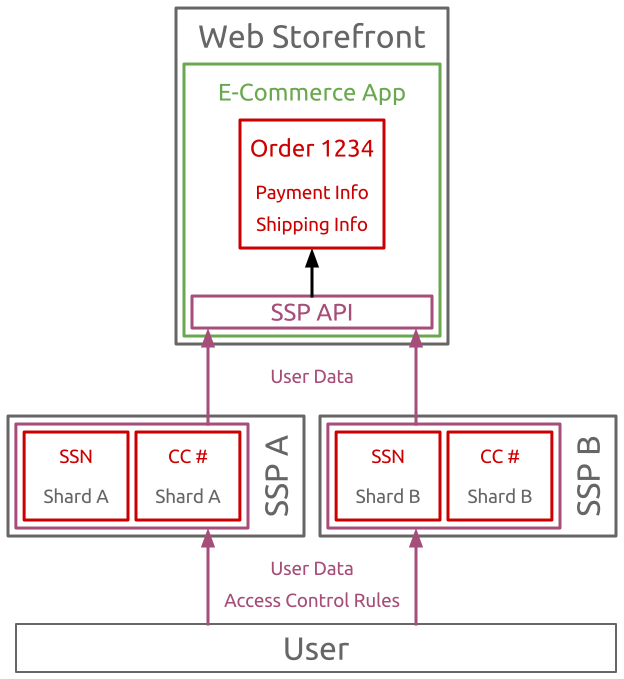
\includegraphics[height=200px]{./figs/out/App-DataRepo.pdf}
  \caption{SSaaS-Backed Personal Data Repo}
  \label{fig:apps-datarepo}
\end{figure}

Moving past traditional applications of storage and encryption, we
could also leverage the SSaaS model to create a dedicated repository
of personal user info (e.g SSN, address, etc). Entering personal user
data on various websites is a common user requirement for placing
orders, creating accounts, etc. This practice is undesirable for
several reason. First, it is highly burdensome: users are continually
forced to reenter the same info and must ensure they keep it up to
date across multiple sites. Second, it distributes a lot of sensitive
user data across a large number of actors in a manner that is very
difficult for a user to control. Instead, I propose that a user shard
their data across several SSPs and then point websites that require it
directly at the SSPs themselves. The user can then specify Access
Control rules with each SSP allowing specific websites access to the
minimum data they require.

Not only does this approach provide a central repository where the
user can enter personal data and keep it up to date (e.g. when
moving), but it also allows the user to limit each site's access to
only certain data and provides an audit trail for the user to track
exactly which sites have accessed which
data. Figure~\ref{fig:apps-datarepo} illustrates such a use case. In
this case, as opposed to the previous encrypted data + SSP-backed
crypto-key use cases, we'll be storing sensitive user data directly
with our SSPs. As such it will be important to shard the data across
multiple SSPs in order to minimize the trust we must place in each
individual SSP.

Such applications could go a long ways toward minimizing the amount of
sensitive personal data we have stored with large number of third
parties in favor of concentrating it on only a handful of SSPs. Doing
so both reduces the trust we must place with any single SSP and ensure
the data is being stored with parties better incentivized to protect
it (see the discussion in Section~\ref{chap:ssaas:trust}).

\section{Communication}

\begin{figure}[t]
  \centering
  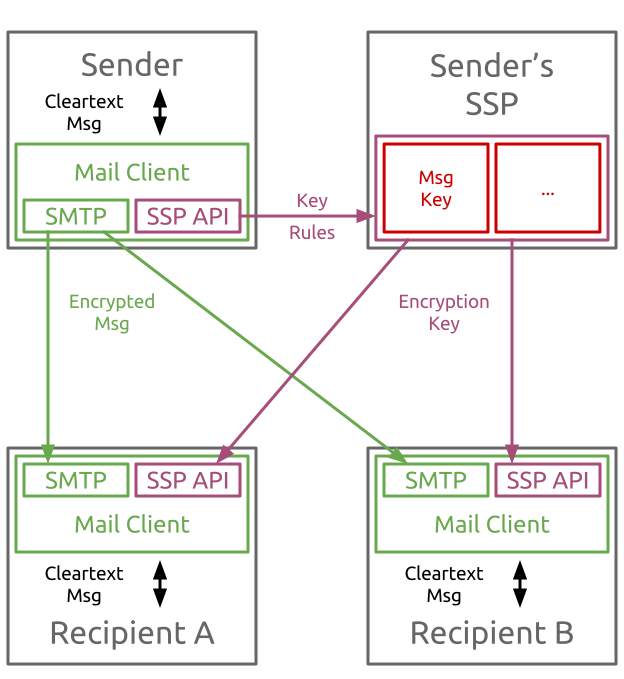
\includegraphics[height=200px]{./figs/out/App-SecureEmail.pdf}
  \caption{SSaaS-Backed Secure Email System}
  \label{fig:apps-secureemail}
\end{figure}

The applications of SSaaS are not limited to data storage. Another
potential area of applications involves secure communication between
two or more parties. Such secure messaging systems are in growing
demand, especially after the Edward Snowden revelations related to US
Government monitoring of email and associated digital communication
systems~\cite{gellman-muscular, greenwald-collect,
  greenwald-prism}. While solutions like GnuPG~\cite{gnupg} exist to
allow users to secure the contents of their mail, their complexity
tends to limit their use to a small subset of advanced
users~\cite{green-challenge, whitten1999}. The secure communication
paradigm could be simplified through the use of SSPs in the SSaaS
model.

Figure~\ref{fig:apps-secureemail} illustrates a potential SSaaS secure
communication use case. In this application, a user's mail client
would encrypt the contents and subject of a user's email prior to
sending it with a locally-generated single-use symmetric encryption
key. The client would then upload this key to the user's SSP where the
user would specify that their intended recipients should have read
access to the key. The user could then send the encrypted mail. When
received, the recipient's mail client would request the required key
from the sender's SSP, providing appropriate credentials to prove
their identity in the process, decrypt, and read the email. This
system would be capable of supporting multi-recipient systems like
newsgroups and would also allow the user to grant read access to
additional users after the fact (e.g. should the recipient wish to
forward the email to an additional trusted party), both capabilities
that traditional public-key based email encryption struggle to
support. Similar applications could be designed for real-time
communication such as chat.

As in previous cases, third party trust can be minimized by sharing
keys across multiple SSPs. Furthermore, such systems could guarantee
some degree of forward secrecy by having the SSP automatically expire
and delete keys after a certain period of time -- something that
traditional email encryption systems struggle to support. Such designs
have the potential to raise the default level of security inherent in
mass digital communication with significantly inconveniencing users.

\section{Authentication}

\subsection{Managed SSH}


\section{Other}

%%  LocalWords:  SSaaS CMAC SSPs SSP's SSP FDE iOS Repo Snowden
